
\section{Evaluation Frameworks and Bias Analysis}
\label{sec:evaluation}

This section presents comprehensive evaluation methodologies specifically designed for feedback-aware recommender systems. We address fundamental challenges in fair comparison across feedback types and present frameworks for bias detection and mitigation.

\begin{figure}[ht]
\centering
\begin{tikzpicture}[scale=0.8, transform shape]
    % Input layer
    \node[rectangle, draw, thick, fill=blue!20, minimum width=8cm, minimum height=1cm, align=center] (input) at (0,8) {\textbf{Recommender System Output}};
    
    % Decision diamond
    \node[regular polygon, regular polygon sides=4, draw, thick, fill=yellow!20, minimum width=2cm, minimum height=1.5cm, align=center] (decision) at (0,6) {Feedback\\Type?};
    
    % Explicit path
    \node[rectangle, draw, fill=red!20, minimum width=3cm, minimum height=0.8cm, align=center] (explicit_metrics) at (-4,4) {Explicit Metrics\\RMSE, MAE};
    \node[rectangle, draw, fill=red!10, minimum width=2.5cm, minimum height=0.6cm, align=center] (rating_pred) at (-4,2.8) {Rating\\Prediction};
    
    % Implicit path
    \node[rectangle, draw, fill=green!20, minimum width=3cm, minimum height=0.8cm, align=center] (implicit_metrics) at (4,4) {Implicit Metrics\\AUC, NDCG};
    \node[rectangle, draw, fill=green!10, minimum width=2.5cm, minimum height=0.6cm, align=center] (ranking) at (4,2.8) {Ranking\\Quality};
    
    % Hybrid path
    \node[rectangle, draw, fill=purple!20, minimum width=3cm, minimum height=0.8cm, align=center] (hybrid_metrics) at (0,4) {Hybrid Metrics\\Composite};
    \node[rectangle, draw, fill=purple!10, minimum width=2.5cm, minimum height=0.6cm, align=center] (multi_task) at (0,2.8) {Multi-task\\Evaluation};
    
    % Common evaluation dimensions
    \node[rectangle, draw, fill=orange!20, minimum width=3cm, minimum height=0.8cm, align=center] (diversity) at (-3,1.5) {Diversity\\Coverage};
    \node[rectangle, draw, fill=orange!20, minimum width=3cm, minimum height=0.8cm, align=center] (novelty) at (0,1.5) {Novelty\\Serendipity};
    \node[rectangle, draw, fill=orange!20, minimum width=3cm, minimum height=0.8cm, align=center] (fairness) at (3,1.5) {Fairness\\Bias Analysis};
    
    % Bias detection
    \node[rectangle, draw, thick, fill=red!30, minimum width=8cm, minimum height=0.8cm, align=center] (bias_detection) at (0,0.2) {\textbf{Bias Detection \& Mitigation}};
    
    % Final evaluation
    \node[rectangle, draw, thick, fill=gray!20, minimum width=8cm, minimum height=0.8cm, align=center] (final) at (0,-1) {\textbf{Comprehensive Performance Report}};
    
    % Arrows
    \draw[thick, ->] (input) -- (decision);
    \draw[->] (decision) -- (-2,5) -- (explicit_metrics);
    \draw[->] (decision) -- (hybrid_metrics);
    \draw[->] (decision) -- (2,5) -- (implicit_metrics);
    
    \draw[->] (explicit_metrics) -- (rating_pred);
    \draw[->] (implicit_metrics) -- (ranking);
    \draw[->] (hybrid_metrics) -- (multi_task);
    
    \draw[->] (rating_pred) -- (diversity);
    \draw[->] (multi_task) -- (novelty);
    \draw[->] (ranking) -- (fairness);
    
    \draw[->] (diversity) -- (bias_detection);
    \draw[->] (novelty) -- (bias_detection);
    \draw[->] (fairness) -- (bias_detection);
    
    \draw[thick, ->] (bias_detection) -- (final);
    
    % Labels
    \node[font=\small] at (-2.5,5.5) {Explicit};
    \node[font=\small] at (0,5.5) {Hybrid};
    \node[font=\small] at (2.5,5.5) {Implicit};
    
\end{tikzpicture}
\caption{Comprehensive Evaluation Framework for Feedback-Aware Recommender Systems}
\label{fig:evaluation_framework}
\end{figure}

Figure~\ref{fig:evaluation_framework} illustrates our systematic evaluation approach that adapts metrics and methodologies based on the underlying feedback mechanism while ensuring comprehensive assessment across multiple quality dimensions.

\subsection{Feedback-Specific Evaluation Challenges}

Traditional evaluation approaches often fail to account for the fundamental differences between implicit and explicit feedback, leading to biased comparisons and misleading conclusions about system performance.

\subsubsection{The Evaluation Gap Problem}
Current evaluation practices treat all recommender systems uniformly, regardless of their underlying feedback mechanisms. This creates several critical issues:

\textbf{Metric Appropriateness}: Metrics designed for explicit feedback (e.g., RMSE for rating prediction) may not adequately capture the effectiveness of implicit feedback systems optimized for ranking.

\textbf{Ground Truth Assumptions}: Implicit feedback systems lack clear negative examples, making standard precision/recall calculations problematic without careful consideration of negative sampling strategies.

\textbf{Temporal Considerations}: Implicit feedback often exhibits different temporal dynamics than explicit feedback, requiring evaluation protocols that account for these differences.

\subsection{Comprehensive Evaluation Framework}

We propose a multi-dimensional evaluation framework that accounts for feedback characteristics while enabling fair comparison across system types.

\subsubsection{Core Evaluation Dimensions}

\textbf{Dimension 1: Predictive Accuracy}
\begin{itemize}
    \item \textit{For Explicit Feedback}: RMSE, MAE for rating prediction
    \item \textit{For Implicit Feedback}: AUC, Hit Ratio, NDCG for ranking
    \item \textit{For Hybrid Systems}: Composite metrics combining both paradigms
\end{itemize}

\textbf{Dimension 2: Ranking Quality}
\begin{itemize}
    \item \textit{Precision@K}: $P@K = \frac{|R@K \cap T|}{K}$
    \item \textit{Recall@K}: $R@K = \frac{|R@K \cap T|}{|T|}$
    \item \textit{NDCG@K}: $NDCG@K = \frac{DCG@K}{IDCG@K}$
    \item \textit{Mean Reciprocal Rank}: $MRR = \frac{1}{|Q|}\sum_{i=1}^{|Q|}\frac{1}{rank_i}$
\end{itemize}

\textbf{Dimension 3: Diversity and Coverage}
\begin{itemize}
    \item \textit{Intra-list Diversity}: Average pairwise dissimilarity within recommendation lists
    \item \textit{Catalog Coverage}: Percentage of items recommended across all users
    \item \textit{User Coverage}: Percentage of users receiving satisfactory recommendations
\end{itemize}

\textbf{Dimension 4: Novelty and Serendipity}
\begin{itemize}
    \item \textit{Novelty}: Average popularity of recommended items (inversely related)
    \item \textit{Serendipity}: Unexpected but relevant recommendations
    \item \textit{Discovery Rate}: New items successfully introduced to users
\end{itemize}

\subsubsection{Feedback-Aware Evaluation Protocols}

\textbf{Protocol 1: Stratified Evaluation by Feedback Type}
\begin{algorithm}[h]
\caption{Feedback-Stratified Evaluation}
\begin{algorithmic}[1]
\STATE Input: Dataset $D$, Feedback types $F = \{f_1, f_2, ..., f_k\}$
\STATE Output: Performance metrics $M = \{m_1, m_2, ..., m_k\}$
\FOR{each feedback type $f_i \in F$}
    \STATE $D_i \leftarrow$ Extract data of type $f_i$ from $D$
    \STATE $Train_i, Test_i \leftarrow$ Split $D_i$ temporally
    \STATE $Model_i \leftarrow$ Train model on $Train_i$
    \STATE $Pred_i \leftarrow$ Generate predictions for $Test_i$
    \STATE $m_i \leftarrow$ Evaluate $Pred_i$ using appropriate metrics for $f_i$
\ENDFOR
\RETURN $M$
\end{algorithmic}
\end{algorithm}

\textbf{Protocol 2: Cross-Feedback Validation}
For hybrid systems, we evaluate performance when feedback types are available in different combinations:
\begin{itemize}
    \item \textit{Full Information}: All feedback types available
    \item \textit{Partial Information}: Subsets of feedback types
    \item \textit{Cold-Start}: No feedback available for new users/items
    \item \textit{Feedback Transition}: Performance when feedback types change over time
\end{itemize}

\subsection{Bias Detection and Analysis Framework}

Bias in recommender systems can significantly impact both system performance and user experience. We provide comprehensive analysis of bias types and detection methodologies.

\subsubsection{Taxonomy of Biases in Feedback-Based Systems}

\begin{figure}[ht]
\centering
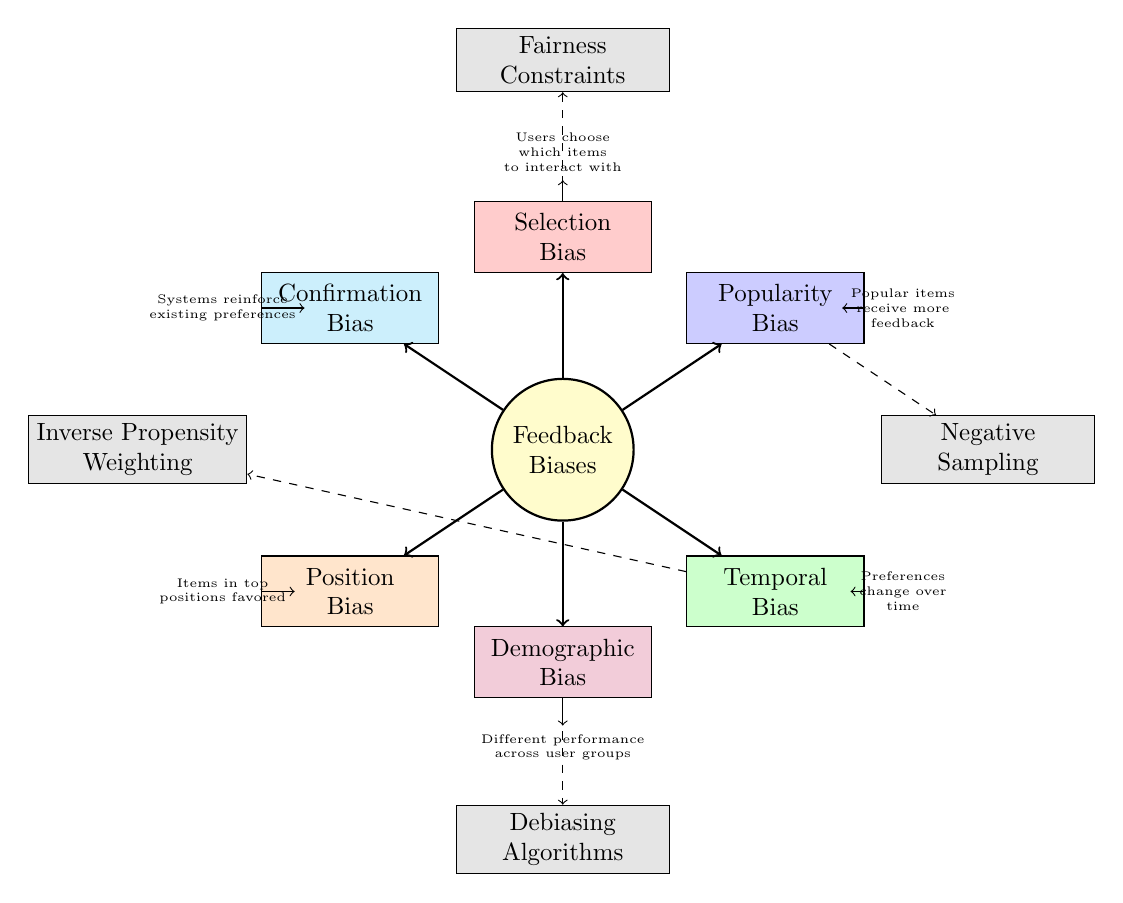
\begin{tikzpicture}[scale=0.9, transform shape]
    % Central node
    \node[circle, draw, thick, fill=yellow!20, minimum size=2cm, align=center] (center) at (0,0) {Feedback\\Biases};
    
    % Bias types around the circle
    \node[rectangle, draw, fill=red!20, minimum width=2.5cm, minimum height=1cm, align=center] (selection) at (0,3) {Selection\\Bias};
    \node[rectangle, draw, fill=blue!20, minimum width=2.5cm, minimum height=1cm, align=center] (popularity) at (3,2) {Popularity\\Bias};
    \node[rectangle, draw, fill=green!20, minimum width=2.5cm, minimum height=1cm, align=center] (temporal) at (3,-2) {Temporal\\Bias};
    \node[rectangle, draw, fill=purple!20, minimum width=2.5cm, minimum height=1cm, align=center] (demographic) at (0,-3) {Demographic\\Bias};
    \node[rectangle, draw, fill=orange!20, minimum width=2.5cm, minimum height=1cm, align=center] (position) at (-3,-2) {Position\\Bias};
    \node[rectangle, draw, fill=cyan!20, minimum width=2.5cm, minimum height=1cm, align=center] (confirmation) at (-3,2) {Confirmation\\Bias};
    
    % Impact descriptions
    \node[align=center, font=\tiny] (sel_desc) at (0,4.2) {Users choose\\which items\\to interact with};
    \node[align=center, font=\tiny] (pop_desc) at (4.8,2) {Popular items\\receive more\\feedback};
    \node[align=center, font=\tiny] (temp_desc) at (4.8,-2) {Preferences\\change over\\time};
    \node[align=center, font=\tiny] (demo_desc) at (0,-4.2) {Different performance\\across user groups};
    \node[align=center, font=\tiny] (pos_desc) at (-4.8,-2) {Items in top\\positions favored};
    \node[align=center, font=\tiny] (conf_desc) at (-4.8,2) {Systems reinforce\\existing preferences};
    
    % Mitigation strategies
    \node[rectangle, draw, fill=gray!20, minimum width=3cm, minimum height=0.7cm, align=center] (mit1) at (-6,0) {Inverse Propensity\\Weighting};
    \node[rectangle, draw, fill=gray!20, minimum width=3cm, minimum height=0.7cm, align=center] (mit2) at (6,0) {Negative\\Sampling};
    \node[rectangle, draw, fill=gray!20, minimum width=3cm, minimum height=0.7cm, align=center] (mit3) at (0,5.5) {Fairness\\Constraints};
    \node[rectangle, draw, fill=gray!20, minimum width=3cm, minimum height=0.7cm, align=center] (mit4) at (0,-5.5) {Debiasing\\Algorithms};
    
    % Arrows from center to bias types
    \draw[thick, ->] (center) -- (selection);
    \draw[thick, ->] (center) -- (popularity);
    \draw[thick, ->] (center) -- (temporal);
    \draw[thick, ->] (center) -- (demographic);
    \draw[thick, ->] (center) -- (position);
    \draw[thick, ->] (center) -- (confirmation);
    
    % Arrows to descriptions
    \draw[->] (selection) -- (sel_desc);
    \draw[->] (popularity) -- (pop_desc);
    \draw[->] (temporal) -- (temp_desc);
    \draw[->] (demographic) -- (demo_desc);
    \draw[->] (position) -- (pos_desc);
    \draw[->] (confirmation) -- (conf_desc);
    
    % Arrows to mitigation strategies
    \draw[dashed, ->] (selection) -- (mit3);
    \draw[dashed, ->] (popularity) -- (mit2);
    \draw[dashed, ->] (temporal) -- (mit1);
    \draw[dashed, ->] (demographic) -- (mit4);
    
\end{tikzpicture}
\caption{Comprehensive Bias Analysis Framework for Feedback-Aware Systems}
\label{fig:bias_analysis}
\end{figure}

Figure~\ref{fig:bias_analysis} illustrates the major sources of bias in feedback-based recommender systems and their corresponding mitigation strategies, emphasizing the need for systematic bias detection and correction across all feedback types.

\textbf{Selection Bias}
Users choose which items to interact with or rate, creating biased training data:
\begin{equation}
P(feedback|item) \neq P(feedback|item, selection)
\end{equation}

\textit{Detection}: Compare feedback distributions with random samples
\textit{Impact}: Underrepresentation of certain item types or user groups

\textbf{Popularity Bias}
Over-representation of popular items in both training data and recommendations:
\begin{equation}
Popularity\_Bias = \frac{\sum_{i \in R} popularity(i)}{|R|} - \frac{\sum_{i \in C} popularity(i)}{|C|}
\end{equation}
where $R$ is the recommendation set and $C$ is the catalog.

\textbf{Temporal Bias}
Changing preferences and item availability over time affecting evaluation:
\begin{equation}
Temporal\_Drift(t) = \frac{||P_t - P_{t-\Delta}||_2}{||P_{t-\Delta}||_2}
\end{equation}
where $P_t$ represents preference distribution at time $t$.

\textbf{Demographic Bias}
Differential performance across user demographics:
\begin{equation}
Fairness\_Gap = \max_{g_i, g_j \in G} |Performance(g_i) - Performance(g_j)|
\end{equation}
where $G$ is the set of demographic groups.

\subsubsection{Bias Mitigation Strategies}

\textbf{For Implicit Feedback Systems}:
\begin{itemize}
    \item \textit{Inverse Propensity Weighting}: Weight observations by inverse of selection probability
    \item \textit{Negative Sampling Strategies}: Carefully select negative examples to reduce bias
    \item \textit{Temporal Debiasing}: Account for time-varying preferences and item popularity
\end{itemize}

\textbf{For Explicit Feedback Systems}:
\begin{itemize}
    \item \textit{Rating Bias Correction}: Normalize for user rating tendencies and item popularity
    \item \textit{Missing Data Imputation}: Use principled approaches for handling missing ratings
    \item \textit{Cross-Validation Strategies}: Ensure representative train/test splits
\end{itemize}

\textbf{For Hybrid Systems}:
\begin{itemize}
    \item \textit{Multi-Objective Optimization}: Balance accuracy and fairness across feedback types
    \item \textit{Bias-Aware Fusion}: Weight feedback sources considering their bias characteristics
    \item \textit{Ensemble Debiasing}: Use diverse models to reduce systematic biases
\end{itemize}

\subsection{Experimental Design Considerations}

\subsubsection{Dataset Requirements and Characteristics}

\textbf{Essential Dataset Properties}:
\begin{itemize}
    \item \textit{Multi-Modal Feedback}: Datasets containing both implicit and explicit signals
    \item \textit{Temporal Information}: Timestamps enabling temporal analysis
    \item \textit{Rich Metadata}: User and item characteristics for bias analysis
    \item \textit{Sufficient Scale}: Adequate size for robust statistical analysis
\end{itemize}

\textbf{Benchmark Datasets for Feedback Research}:
\begin{table}[h]
\centering
\caption{Key Datasets for Feedback-Aware Evaluation}
\label{tab:datasets}
\begin{tabular}{@{}lcccc@{}}
\toprule
Dataset & Domain & Implicit & Explicit & Users/Items \\
\midrule
Amazon Product & E-commerce & \checkmark & \checkmark & 8M/2.3M \\
Netflix & Streaming & \checkmark & \checkmark & 480K/17K \\
Last.fm & Music & \checkmark & \checkmark & 360K/160K \\
Yelp & Reviews & \checkmark & \checkmark & 1.6M/200K \\
MovieLens-25M & Movies & \checkmark & \checkmark & 280K/58K \\
\bottomrule
\end{tabular}
\end{table}

\subsubsection{Statistical Testing and Significance}

\textbf{Appropriate Statistical Tests}:
\begin{itemize}
    \item \textit{Wilcoxon Signed-Rank Test}: For non-parametric paired comparisons
    \item \textit{McNemar's Test}: For comparing binary classification performance
    \item \textit{Bootstrap Confidence Intervals}: For robust uncertainty estimation
    \item \textit{Multiple Comparison Correction}: Bonferroni or FDR correction for multiple metrics
\end{itemize}

\textbf{Effect Size Measures}:
Beyond statistical significance, we emphasize practical significance:
\begin{equation}
Cohen's\_d = \frac{\mu_1 - \mu_2}{\sqrt{\frac{\sigma_1^2 + \sigma_2^2}{2}}}
\end{equation}

\subsection{Advanced Evaluation Methodologies}

\subsubsection{Counterfactual Evaluation}
For scenarios where online A/B testing is impractical:

\textbf{Inverse Propensity Scoring (IPS)}:
\begin{equation}
\hat{R}_{IPS} = \frac{1}{n}\sum_{i=1}^n \frac{r_i \cdot \mathbf{1}[a_i = \pi(x_i)]}{p(a_i|x_i)}
\end{equation}
where $r_i$ is the reward, $a_i$ is the action, $\pi(x_i)$ is the policy, and $p(a_i|x_i)$ is the propensity score.

\textbf{Doubly Robust Estimation}:
Combines direct method and IPS for more robust evaluation:
\begin{equation}
\hat{R}_{DR} = \hat{R}_{DM} + \frac{1}{n}\sum_{i=1}^n \frac{\mathbf{1}[a_i = \pi(x_i)]}{p(a_i|x_i)}(r_i - \hat{r}(x_i, a_i))
\end{equation}

\subsubsection{Multi-Stakeholder Evaluation}
Modern recommender systems must balance multiple stakeholder interests:

\textbf{User Satisfaction Metrics}:
\begin{itemize}
    \item \textit{Click-Through Rate}: Immediate engagement
    \item \textit{Dwell Time}: Content consumption depth
    \item \textit{Return Rate}: Long-term user retention
    \item \textit{Explicit Satisfaction}: Direct user feedback on recommendations
\end{itemize}

\textbf{Platform Metrics}:
\begin{itemize}
    \item \textit{Catalog Turnover}: Rate of new item discovery
    \item \textit{Revenue Impact}: Business value of recommendations
    \item \textit{Computational Efficiency}: Resource utilization
\end{itemize}

\textbf{Creator/Provider Metrics}:
\begin{itemize}
    \item \textit{Exposure Fairness}: Equal opportunity for item visibility
    \item \textit{Long-tail Coverage}: Support for niche content
    \item \textit{Creator Diversity}: Representation across different providers
\end{itemize}

\subsection{Reproducibility and Standardization}

\subsubsection{Evaluation Framework Implementation}
To promote reproducible research, we provide:

\begin{itemize}
    \item \textbf{Standardized Metrics}: Reference implementations of feedback-aware metrics
    \item \textbf{Evaluation Protocols}: Step-by-step procedures for different scenarios
    \item \textbf{Bias Detection Tools}: Automated analysis of common bias types
    \item \textbf{Statistical Testing Suite}: Appropriate tests for different comparison scenarios
\end{itemize}

\subsubsection{Best Practices for Reporting Results}

\textbf{Essential Reporting Elements}:
\begin{itemize}
    \item \textit{Dataset Characteristics}: Detailed description of feedback types and distributions
    \item \textit{Evaluation Protocol}: Clear specification of train/test procedures
    \item \textit{Statistical Testing}: Significance tests and confidence intervals
    \item \textit{Bias Analysis}: Assessment of potential biases and mitigation strategies
    \item \textit{Computational Requirements}: Resource usage and scalability considerations
\end{itemize}

This comprehensive evaluation framework enables fair comparison of recommender systems across different feedback types while accounting for their inherent characteristics and potential biases. By adopting these methodologies, the research community can make more reliable progress in developing effective feedback-aware recommendation systems.

\begin{itemize}
    \item \textbf{Implicit feedback} often uses binary relevance (clicked/not clicked), favoring ranking accuracy over absolute preference strength.
    \item \textbf{Explicit feedback} incorporates preference strength, allowing for more nuanced evaluation of recommendation quality.
    \item \textbf{Hybrid approaches} require careful calibration to balance ranking and rating prediction objectives.
\end{itemize}

The mathematical formulations reveal important differences:

\begin{equation}
\text{Precision@K} = \frac{|\{i \in \text{top-K} \cap \text{relevant}\}|}{K}
\label{eq:precision_k}
\end{equation}

\begin{equation}
\text{NDCG@K} = \frac{1}{|U|} \sum_{u \in U} \frac{\sum_{i=1}^K \frac{rel_{u,i}}{log_2(i+1)}}{\sum_{i=1}^{|REL_u|} \frac{1}{log_2(i+1)}}
\label{eq:ndcg_k}
\end{equation}

where $rel_{u,i}$ represents relevance scores that differ significantly between implicit (binary) and explicit (graded) feedback.

\subsubsection{Rating Prediction Metrics}
Root Mean Square Error (RMSE) and Mean Absolute Error (MAE) evaluate explicit rating predictions:

\begin{equation}
\text{RMSE} = \sqrt{\frac{1}{|R|} \sum_{(u,i) \in R} (\hat{r}_{ui} - r_{ui})^2}
\label{eq:rmse}
\end{equation}

\begin{equation}
\text{MAE} = \frac{1}{|R|} \sum_{(u,i) \in R} |\hat{r}_{ui} - r_{ui}|
\label{eq:mae}
\end{equation}

These metrics are less applicable to implicit feedback, which lacks ground-truth ratings, necessitating alternative evaluation approaches.

\subsubsection{Area Under the Curve (AUC) Metrics}
For implicit feedback evaluation, AUC-based metrics provide robust ranking assessment:

\begin{equation}
\text{AUC} = \frac{1}{|U|} \sum_{u \in U} \frac{1}{|I_u^+||I_u^-|} \sum_{i^+ \in I_u^+} \sum_{i^- \in I_u^-} \mathbb{I}(\hat{r}_{ui^+} > \hat{r}_{ui^-})
\label{eq:auc}
\end{equation}

where $I_u^+$ and $I_u^-$ represent positive and negative feedback items for user $u$.

\subsection{Evaluation Biases and Challenges}

\subsubsection{Dataset Biases}
Public datasets exhibit various biases that affect evaluation reliability:

\begin{table}[h]
\centering
\caption{Evaluation Biases in Different Feedback Types}
\label{tab:evaluation_biases}
\begin{tabular}{@{}lccc@{}}
\toprule
Bias Type & Implicit Feedback & Explicit Feedback & Mitigation Strategies \\
\midrule
Popularity Bias & High (rich-get-richer) & Moderate & Inverse propensity scoring \\
Position Bias & Very High & Moderate & Position debiasing, randomization \\
Selection Bias & Low & Very High & Inverse propensity weighting \\
Confirmation Bias & Moderate & High & Counterfactual evaluation \\
Temporal Bias & High & Moderate & Time-aware validation \\
Demographic Bias & Moderate & High & Fairness-aware evaluation \\
\bottomrule
\end{tabular}
\end{table}

\subsubsection{User Behavior Interpretations}
Implicit feedback interpretations can be misleading:

\begin{itemize}
    \item \textbf{Engagement vs. Interest}: Long watch times may indicate engagement or involuntary attention (e.g., background TV)
    \item \textbf{Contextual Influences}: Clicks may result from curiosity, social pressure, or algorithmic manipulation
    \item \textbf{Behavioral Variability}: User interaction patterns vary significantly across demographics and contexts
    \item \textbf{False Negatives}: Lack of interaction doesn't necessarily indicate lack of interest
\end{itemize}

Explicit feedback, while clearer, has its own interpretation challenges:

\begin{itemize}
    \item \textbf{Mood-Dependent Ratings}: Emotional state influences rating consistency
    \item \textbf{Social Desirability Bias}: Users provide socially acceptable rather than genuine opinions
    \item \textbf{Scale Interpretation Variance}: Different users interpret rating scales differently
    \item \textbf{Recency Effects}: Recent experiences disproportionately influence feedback
\end{itemize}

\subsection{Advanced Evaluation Frameworks}

\subsubsection{Novelty and Diversity Metrics}

Beyond accuracy, diversity and novelty are crucial for user satisfaction:

\begin{equation}
\text{Novelty} = -\log_2(\text{popularity}(i))
\label{eq:novelty}
\end{equation}

\begin{equation}
\text{Diversity} = 1 - \frac{\sum_{i,j \in L} s(i,j)}{|L|(|L|-1)}
\label{eq:diversity}
\end{equation}

where $s(i,j)$ measures similarity between recommended items and $L$ is the recommendation list.

\subsubsection{Serendipity Metrics}

Measuring unexpected relevant recommendations:

\begin{equation}
\text{Serendipity} = \frac{1}{|U|} \sum_u \frac{|\{i \in L_u | rel(u,i) \land unexpected(u,i)\}|}{|L_u|}
\label{eq:serendipity}
\end{equation}

\subsubsection{Coverage Metrics}

Assessing catalog utilization:

\begin{equation}
\text{Catalog Coverage} = \frac{|\bigcup_u L_u|}{|\mathcal{I}|}
\label{eq:coverage}
\end{equation}

\begin{equation}
\text{User Coverage} = \frac{|\{u | |L_u| > 0\}|}{|U|}
\label{eq:user_coverage}
\end{equation}

\subsection{User-Centric Evaluation Methods}

\subsubsection{A/B Testing and Online Evaluation}

Real-world performance assessment through controlled experiments:

\begin{itemize}
    \item \textbf{Interleaving Methods}: Comparing ranking algorithms by interleaving recommendations
    \item \textbf{Multi-Armed Bandit Evaluation}: Online learning-based evaluation protocols
    \item \textbf{Counterfactual Evaluation}: Estimating performance under different conditions
\end{itemize}

\subsubsection{User Studies and Surveys}

Qualitative assessment of user experience:

\begin{itemize}
    \item \textbf{Satisfaction Surveys}: Measuring perceived recommendation quality
    \item \textbf{Trust Assessments}: Evaluating system credibility and transparency
    \item \textbf{Behavioral Metrics}: Task completion rates and engagement patterns
    \item \textbf{Longitudinal Studies}: Tracking user behavior over extended periods
\end{itemize}

\subsubsection{Eye-Tracking and Physiological Measures}

Advanced user response measurement:

\begin{itemize}
    \item \textbf{Fixation Duration}: Measuring attention to recommended items
    \item \textbf{Pupil Dilation}: Indicating cognitive load and interest intensity
    \item \textbf{Heart Rate Variability}: Assessing emotional responses to recommendations
\end{itemize}

\subsection{Bias Mitigation in Evaluation}

\subsubsection{Debiasing Techniques}

Addressing evaluation biases through statistical corrections:

\begin{itemize}
    \item \textbf{Inverse Propensity Scoring}: Correcting for selection biases in explicit feedback
    \item \textbf{Position Bias Debiasing}: Accounting for presentation order effects
    \item \textbf{Popularity Bias Correction}: Balancing evaluation across item popularity levels
    \item \textbf{Temporal Debiasing}: Handling temporal distribution shifts in feedback
\end{itemize}

\subsubsection{Fairness-Aware Evaluation}

Ensuring equitable performance across user groups:

\begin{equation}
\text{Demographic Parity} = \max_g \left| \frac{|\{u \in g | \text{satisfied}(u)\}|}{|g|} - \frac{|\{u \notin g | \text{satisfied}(u)\}|}{|U \setminus g|} \right|
\label{eq:demographic_parity}
\end{equation}

\subsection{Dataset Construction and Benchmarking}

\subsubsection{Synthetic Dataset Generation}

Creating controlled evaluation environments:

\begin{itemize}
    \item \textbf{Simulation-Based Datasets}: Generating feedback based on known user preferences
    \item \textbf{Counterfactual Datasets}: Creating "what-if" scenarios for causal evaluation
    \item \textbf{Multi-Behavior Datasets}: Capturing diverse feedback types simultaneously
\end{itemize}

\subsubsection{Cross-Domain Evaluation}

Assessing generalizability across different contexts:

\begin{itemize}
    \item \textbf{Domain Adaptation Metrics}: Measuring performance transfer between domains
    \item \textbf{Out-of-Distribution Evaluation}: Testing robustness to novel scenarios
    \item \textbf{Meta-Evaluation}: Evaluating evaluation metrics themselves
\end{itemize}

\subsection{Statistical Rigor and Reproducibility}

\subsubsection{Confidence Intervals and Significance Testing}

Ensuring reliable performance comparisons:

\begin{equation}
\text{Confidence Interval} = \bar{x} \pm z \cdot \frac{\sigma}{\sqrt{n}}
\label{eq:confidence_interval}
\end{equation}

\subsubsection{Reproducibility Challenges}

Addressing evaluation variability:

\begin{itemize}
    \item \textbf{Algorithmic Randomness}: Controlling stochastic elements in model training
    \item \textbf{Dataset Splits}: Ensuring consistent train/test/validation partitions
    \item \textbf{Hyperparameter Sensitivity}: Reporting performance across parameter ranges
    \item \textbf{Computational Reproducibility}: Managing hardware and software dependencies
\end{itemize}

\subsection{Domain-Specific Evaluation Considerations}

\subsubsection{E-commerce Evaluation}

Focusing on conversion and revenue metrics:

\begin{itemize}
    \item \textbf{Conversion Rate}: Percentage of recommendations leading to purchases
    \item \textbf{Revenue per User}: Economic impact of recommendation strategies
    \item \textbf{Cart Completion Rate}: Effectiveness in reducing abandonment
    \item \textbf{Cross-Sell Performance}: Success in suggesting complementary products
\end{itemize}

\subsubsection{Content Streaming Evaluation}

Emphasizing engagement and retention:

\begin{itemize}
    \item \textbf{Watch Time}: Total engagement duration with recommended content
    \item \textbf{Completion Rate}: Percentage of content consumed to completion
    \item \textbf{Skip Rate}: Negative feedback through content abandonment
    \item \textbf{Return Visits}: Long-term user retention and loyalty
\end{itemize}

\subsubsection{Social Media Evaluation}

Measuring network and information effects:

\begin{itemize}
    \item \textbf{Viral Coefficient}: Amplification of content through social sharing
    \item \textbf{Engagement Rate}: Likes, comments, and shares per recommendation
    \item \textbf{Information Diversity}: Balance between personalized and diverse content
    \item \textbf{Polarization Metrics}: Assessing filter bubble effects
\end{itemize}

\subsection{Temporal and Dynamic Evaluation}

\subsubsection{Concept Drift Detection}

Monitoring performance stability over time:

\begin{equation}
\text{Drift Score} = \frac{1}{T} \sum_{t=1}^T |\mu_{t} - \mu_{t-1}|
\label{eq:drift_score}
\end{equation}

where $\mu_t$ represents performance metrics at time $t$.

\subsubsection{Adaptive Evaluation Protocols}

Dynamic assessment methods for evolving systems:

\begin{itemize}
    \item \textbf{Online Learning Evaluation}: Continuous performance monitoring
    \item \textbf{Contextual Evaluation}: Performance assessment under different conditions
    \item \textbf{Multi-Horizon Evaluation}: Short-term vs. long-term impact assessment
\end{itemize}

\subsection{Future Evaluation Directions}

Emerging evaluation paradigms include:

\begin{itemize}
    \item \textbf{Causal Evaluation}: Understanding causal relationships between recommendations and outcomes
    \item \textbf{Multimodal Evaluation}: Assessing performance across different feedback modalities
    \item \textbf{Human-AI Collaborative Evaluation}: Combining automated metrics with human judgment
    \item \textbf{Sustainable Evaluation}: Measuring environmental and social impact of recommendation systems
\end{itemize}

This comprehensive evaluation framework ensures that recommender systems are assessed appropriately for their feedback characteristics, providing reliable and meaningful performance comparisons across different approaches and domains.
